
\documentclass[10pt,a4paper]{article}

\usepackage[a4paper,top=18mm,bottom=18mm,left=18mm,right=18mm]{geometry}
\usepackage[T1]{fontenc}
\usepackage{lmodern,microtype}
\usepackage{amsmath,amssymb,mathtools,bm}
\usepackage{xcolor,booktabs,tabularx,array,enumitem,multicol,graphicx}
\usepackage{tikz}
\usetikzlibrary{arrows.meta,positioning,calc}
\usepackage[most]{tcolorbox}
\usepackage{fancyhdr,hyperref}
\definecolor{ink}{HTML}{24354B}
\definecolor{accent}{HTML}{135E77}
\definecolor{pale}{HTML}{F1F7F8}
\hypersetup{colorlinks=true,linkcolor=accent,urlcolor=accent,pdfauthor={PHYS4055 revision notes}}
\setlength{\parindent}{0pt}
\setlength{\parskip}{4pt}
\setlength{\emergencystretch}{3em}
\setlist{leftmargin=*,topsep=2pt,itemsep=1pt}
\AtBeginDocument{\color{ink}}
\pagestyle{fancy}
\fancyhf{}
\fancyhead[L]{\footnotesize PHYS4055 \textbar\ Exam Revision}
\fancyhead[R]{\footnotesize 2026 \textbar\ Open-book notes}
\fancyfoot[C]{\footnotesize\thepage}
\renewcommand{\headrulewidth}{0.3pt}
\newcommand{\ket}[1]{\left\lvert #1\right\rangle}
\newcommand{\bra}[1]{\left\langle #1\right\rvert}
\newcommand{\braket}[2]{\left\langle #1\middle\vert #2\right\rangle}
\newcommand{\mel}[3]{\left\langle #1\middle\vert #2\middle\vert #3\right\rangle}
\newcommand{\diff}{\mathrm{d}}
\newcommand{\ii}{\mathrm{i}}
\newcommand{\e}{\mathrm{e}}
\newtcolorbox{methodbox}{colback=pale,colframe=accent!50!white,boxrule=0.4pt,arc=1mm,before skip=5pt,after skip=5pt}
\newtcolorbox{cautionbox}{colback=white,colframe=black!20,boxrule=0.4pt,arc=1mm,before skip=5pt,after skip=5pt}

\hypersetup{pdftitle={PHYS4055 - Course Overview}}
\title{\textcolor{accent}{PHYS4055: Course Overview}\\[2mm]\large Atomic structure, angular momentum and optical transitions}
\author{2026 open-book revision \textbar\ evolving working document}
\date{12 November 2026}
\begin{document}
\maketitle
\begin{cautionbox}
This is a starter overview, not an audited reproduction of the 2026 syllabus.
Complete and check it against the lectures and past papers as they are uploaded.
\end{cautionbox}
\tableofcontents
\clearpage

\section{Angular momentum: the big picture}
For a state \(\ket{j,m}\), the commuting operators \(\hat J^2\) and \(\hat J_z\) have
\[
\hat J^2\ket{j,m}=\hbar^2 j(j+1)\ket{j,m},\qquad
\hat J_z\ket{j,m}=\hbar m\ket{j,m}.
\]
The projections are \(m=-j,-j+1,\ldots,j\), giving \(2j+1\) magnetic substates.
\subsection{Adding two angular momenta}
If \(\hat{\mathbf J}=\hat{\mathbf J}_1+\hat{\mathbf J}_2\), then
\[
j=|j_1-j_2|,\ |j_1-j_2|+1,\ldots,j_1+j_2.
\]
The uncoupled basis \(\ket{j_1m_1}\ket{j_2m_2}\) and the coupled
basis \(\ket{(j_1j_2)jm}\) describe the same space:
\[
\ket{(j_1j_2)jm}
=\sum_{m_1+m_2=m}\langle j_1m_1,j_2m_2|jm\rangle
\ket{j_1m_1}\ket{j_2m_2}.
\]
\begin{methodbox}
\textbf{Exam method:} use the triangle rule to list allowed \(j\).
Check \(\sum_j(2j+1)=(2j_1+1)(2j_2+1)\).
\end{methodbox}
\subsection{Atomic quantum numbers and terms}
For one electron, \(\mathbf j=\mathbf l+\mathbf s\), where \(s=\tfrac12\).
For many-electron LS coupling,
\(\mathbf L=\sum_i\mathbf l_i\), \(\mathbf S=\sum_i\mathbf s_i\),
and \(\mathbf J=\mathbf L+\mathbf S\). A term is written
\[
{}^{2S+1}L_J,\qquad L=0,1,2,3,4\leftrightarrow S,P,D,F,G.
\]
The nuclear spin is \(I\); hyperfine angular momentum is
\(\mathbf F=\mathbf I+\mathbf J\). State which coupling scheme is valid.


\section{Hyperfine structure and magnetic fields}
The magnetic-dipole hyperfine Hamiltonian is
\[
\hat H_{\mathrm{hfs}}=\frac{A}{\hbar^2}\hat{\mathbf I}\cdot\hat{\mathbf J}.
\]
With \(\mathbf F=\mathbf I+\mathbf J\), squaring gives
\(\mathbf F^2=\mathbf I^2+\mathbf J^2+2\mathbf I\cdot\mathbf J\).
Hence the hyperfine energy is
\[
\boxed{E_F=\frac A2[F(F+1)-I(I+1)-J(J+1)].}
\]
This expression treats the magnetic-dipole interaction. An electric-quadrupole
hyperfine correction can be present where angular momenta permit it.
\subsection{Worked level pattern: \(I=\frac52,\ J=\frac12\)}
Possible totals are \(F=2,3\), with \(2F+1=5,7\) states:
\[
E_2=\frac A2\left(6-\frac{35}{4}-\frac34\right)=-\frac{7A}{4},
\qquad
E_3=\frac A2\left(12-\frac{35}{4}-\frac34\right)=\frac{5A}{4}.
\]
Thus \(\Delta E=E_3-E_2=3A\). The total count
\(5+7=(2I+1)(2J+1)=12\) checks completeness. For \(A>0\):
\begin{center}
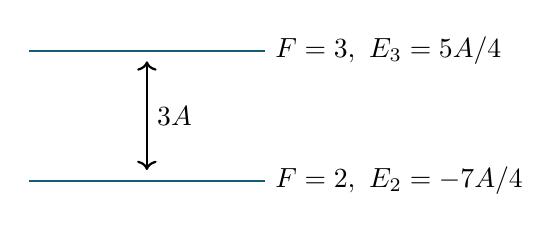
\begin{tikzpicture}[x=1cm,y=0.75cm]
\draw[thick,accent] (0,2.5)--(3,2.5) node[right,black] {$F=3,\ E_3=5A/4$};
\draw[thick,accent] (0,.3)--(3,.3) node[right,black] {$F=2,\ E_2=-7A/4$};
\draw[<->,thick] (1.5,.48)--node[right] {$3A$}(1.5,2.32);
\end{tikzpicture}
\end{center}
For \(A<0\), the energy ordering reverses.
\subsection{Magnetic field regimes}
At weak magnetic fields, \(F,m_F\) are useful quantum numbers:
the linear Zeeman shift is approximately \(\Delta E=g_F\mu_Bm_FB\)
(neglecting small nuclear corrections when appropriate).
At sufficiently strong fields the hyperfine coupling is perturbed,
and \(m_I,m_J\) are more natural labels (hyperfine Paschen--Back regime).
\begin{cautionbox}
Always decide whether the field is weak or strong relative to the hyperfine
splitting \emph{before} selecting the basis.
\end{cautionbox}


\section{Spherical tensors and Wigner--Eckart}
A rank-\(k\) irreducible spherical tensor \(T_q^{(k)}\) has
\(2k+1\) components \(q=-k,\dots,k\). Rank 1 behaves as a vector;
rank 2 has five quadrupole-like components. The Wigner--Eckart theorem
separates angular geometry from dynamics:
\[
\boxed{\langle j'm'|T_q^{(k)}|jm\rangle
=(-1)^{j'-m'}
\begin{pmatrix}j'&k&j\\-m'&q&m\end{pmatrix}
\langle j'\Vert T^{(k)}\Vert j\rangle.}
\]
The \(3j\) symbol enforces \(m'=m+q\), the triangle rule
\(|j-j'|\le k\le j+j'\), and allowed integer/half-integer sums.
A nonzero \(3j\) does \emph{not} guarantee that the reduced matrix
element, and hence the transition, is nonzero.

\subsection{A simple \(3j\) symbol}
Adding angular momentum zero changes nothing:
\(\langle0,0;1,0|1,0\rangle=1\). Hence
\[
\begin{pmatrix}0&1&1\\0&0&0\end{pmatrix}
=\frac{(-1)^{0-1+0}}{\sqrt{2(1)+1}}
\langle0,0;1,0|1,0\rangle=-\frac1{\sqrt3}.
\]

\section{Electromagnetic multipoles and parity}
Electric multipole \(Ek\) has rank \(k\), parity \((-1)^k\).
Magnetic multipole \(Mk\) has rank \(k\), parity \((-1)^{k+1}\).
Both require the angular-momentum triangle rule and projection rule.

\begin{center}
\begin{tabularx}{\linewidth}{@{}lclX@{}}
\toprule
Type & Rank & Operator parity & Common orbital screening (single electron)\\
\midrule
E1 & 1 & odd & Opposite-parity orbitals; \(\Delta l=\pm1\)\\
M1 & 1 & even & Same parity; commonly \(\Delta l=0\)\\
E2 & 2 & even & Same parity; \(\Delta l=0,\pm2\), plus triangle rule\\
\bottomrule
\end{tabularx}
\end{center}
For E1, \(\Delta J=0,\pm1\) but \(J=0\leftrightarrow J'=0\)
is forbidden. For E2, \(|J'-J|\le2\le J'+J\); listing
\(\Delta J=0,\pm1,\pm2\) without this triangle condition is incomplete.
\begin{methodbox}
\textbf{Exam method:} identify \(Ek/Mk\); check parity, triangle and
projection rules; apply the specified spin/orbital assumptions;
then calculate the \(3j\) and reduced/radial elements.
\end{methodbox}


\section{Equivalent electrons and Hund's rules}
For two equivalent \(d\) electrons (\(d^2\)), antisymmetry permits
\[
{}^3F_{2,3,4},\quad {}^3P_{0,1,2},\quad
{}^1G_4,\quad {}^1D_2,\quad {}^1S_0.
\]
The microstate count is
\[
(3\times7)+(3\times3)+(1\times9)+(1\times5)+(1\times1)
=45=\binom{10}{2}.
\]
Hund's first rule favours maximum \(S\); second favours maximum \(L\)
within a multiplicity; third favours the smallest \(J\) for a less-than-half-full
shell. Thus the simple LS-coupled ground-state prediction for \(d^2\)
is \({}^3F_2\). Do not assume Hund's rules uniquely order every
other term: compare to experimental level data.

\section{Radial structure and nuclear-size effects}
For a central potential,
\(\psi_{nlm}(r,\theta,\phi)=R_{nl}(r)Y_{lm}(\theta,\phi)\)
and \(\int_0^\infty|R_{nl}|^2r^2\,\diff r=1\).
The alternative radial function \(u_{nl}(r)=rR_{nl}(r)\) satisfies
\(\int_0^\infty|u_{nl}|^2\,\diff r=1\).
A small change in a central potential can be estimated by first-order
perturbation theory:
\[
\Delta E_{nlm}^{(1)}
=\int\psi_{nlm}^*(\mathbf r)\,\Delta V(r)\,
\psi_{nlm}(\mathbf r)\,\diff^3r.
\]
For a spherically symmetric perturbation the angular integral is unity.
Small-\(r\) contributions matter particularly for orbitals with density
at the nucleus.

\section{E1 dipole matrix elements and radiative lifetimes}
The dipole matrix element factors into angular and radial pieces;
the radial part for \(R\)-normalisation is
\[
\int_0^\infty R_{n_fl_f}^*(r)\,r\,R_{n_il_i}(r)\,r^2\,\diff r.
\]
For specific non-degenerate initial and final states in vacuum,
the spontaneous E1 rate in SI units is
\[
A_{i\to f}=\frac{\omega_{if}^3}{3\pi\epsilon_0\hbar c^3}
\left|\langle f|\hat{\mathbf d}|i\rangle\right|^2,
\quad \hat{\mathbf d}=-e\hat{\mathbf r}.
\]
Treat sums/averages over magnetic substates consistently.
The lifetime includes \emph{all} allowed downward decay channels:
\[
\boxed{\tau_i=\left(\sum_{f:E_f<E_i} A_{i\to f}\right)^{-1}.}
\]
Atomic unit of time: \(t_{\mathrm{au}}\simeq2.418884\times10^{-17}\,\mathrm s\).
\begin{cautionbox}
Using \(u(r)\) in an integral derived for \(R(r)\) introduces incorrect
factors of \(r\). Check radial normalisation and unit conversion.
\end{cautionbox}

\end{document}
